\documentclass[a4paper, 12pt]{article}
\usepackage[slovene]{babel}
\usepackage[utf8]{inputenc}
\usepackage[T1]{fontenc}
\setlength{\parindent}{0px}
\setlength{\parskip}{10px}
%standard

\usepackage{listings}
\usepackage{color}
\usepackage{amssymb}
\usepackage{tikz}
\usepackage{pgfplots}
\usetikzlibrary{patterns}
\pgfplotsset{width=7cm, compat=1.10}
\usepgfplotslibrary{fillbetween}

\usepackage{etoolbox}
\patchcmd{\abstractname}{Povzetek}{Pomembno}{}{}

\title{Avditorne vaje za Programiranje II}
\author{Matej Blagšič}

\begin{document}
%--------------------------------------------
\definecolor{dkgreen}{rgb}{0,0.6,0}
\definecolor{gray}{rgb}{0.5,0.5,0.5}
\definecolor{mauve}{rgb}{0.58,0,0.82}
\definecolor{lgray}{RGB}{250,250,250}
%--------------------------------------------
	\lstset{
		frame=l,%single
		language=C,
		aboveskip=3mm,
		belowskip=3mm,
		showstringspaces=false,
		columns=flexible,
		basicstyle={\small\ttfamily},
		numbers=none,
		numberstyle=\tiny\color{gray},
		keywordstyle=\color{blue},
		commentstyle=\color{dkgreen},
		stringstyle=\color{mauve},
		breaklines=true,
		breakatwhitespace=true,
		tabsize=4,
		backgroundcolor=\color{lgray},
		moredelim=**[is][\color{dkgreen}]{@}{@}
	}
%-------------------------------------------

%-------------------------------------------
	\maketitle
	\thispagestyle{empty}
	\pagebreak
	\setcounter{page}{1}
	\tableofcontents
	\pagebreak
%-----------------------------------Tu naprej

\begin{center}
\textbf{Pomembno}
\end{center}
Te vaje so direktno iz pouka. Koda morda ni identična od te asistena, ampak deluje enako. Prav tako je komentirana in obrazložena skupaj z navodili in opazkami za lažje razumevanje kode. Prav tako se sklicujem in že tu pozivam, da si pogledaš zapiske iz pouka, ki so kot nekakšen učbenik. Notri je snov, teorija in primeri iz pouka. Prijetno branje in učenje želim!

\section{Vaja}
/empty/
\section{Vaja}

\underline{Izračunaj $\int_{x_0}^{x_1}\, 2x^2-5x\, dx$. Rezultat preveri analitično.}	\

Če analitično integriramo itegral, dobimo: $\int_{x_0}^{x_1}\, 2x^2-5x\, dx = 2\frac{x_1^3}3-5\frac{x_0^2}2$\

Sedaj spišimo kodo:
\begin{lstlisting}
int main(){
	float x, x0, x1;
	float dx = 0.0000001;
	float integral = 0;
	printf("vnesi spodno mejo");
	scanf("%f",&x0);
	printf("Vnesi zgornjo mejo");
	scanf("%f",&x1);

	for(x=x0; x<x1;x+=dx){
		integral += dx*(2*x*x-5*x);
	}

	printf("Integral znasa: %f\n", integral);
	return 0;
}
\end{lstlisting}
Pri programu nam spremenljivka dx sporoči, kako širok del območja integrira. Manjša, kot je cifra, bolj natančno izračuna. x0 in x1 sta spodnja in zgornja meja integracije, x pa je spremenjivka, ki jo premikamo po intervalu za dx razdaljo in seštevamo pravokotnike.
	
\begin{figure}[!htbp]
	\centering
	\caption{Integracije funkcije na intervalu $[a, b]$}
	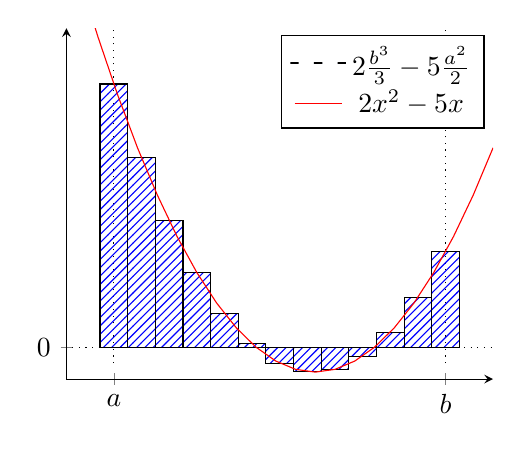
\begin{tikzpicture}
	\begin{axis}[axis lines=left,xmin=-4,xmax=5,ymin=-4,ymax=40,ytick={0}, yticklabel={$0$},xtick={-3,4},xticklabels={$a$,$b$}]
		\addplot[dotted]{0};
		\addplot+[mark=none, dotted, color=black] coordinates {(-3, -2)(-3,40)};
		\addplot+[mark=none, dotted, color=black] coordinates {(4, -2)(4,40)};
		\addplot[domain=-3:4, ybar, samples=13, pattern = north east lines, pattern color=blue]{2*x*x-5*x};
		\addplot[color = red]{2*x*x-5*x};
		\legend{,,,$ 2\frac{b^3}3-5\frac{a^2}2$, $2x^2-5x$}
	\end{axis}
	\end{tikzpicture}
\end{figure}
	
\section{Vaja}
\subsection*{1. naloga}

\underline{Napiši program, ki izpiše in izračuna faktorielo(fakulteta) nekega števila(1-20)}\

Pri temu programu spoznamo omejitve velikosti spremenljivk. Pomemno je, da so števila, ki jih hočemo hraniti in predstavljani v polni natančnosti ne presegajo velikosti spremenljivke. Če ne, potem se prične pačenje podatkov. Vidimo, da lahko uporabimo izrad long long in s tem povečamo obseh navadnega long tipa. Podobno lahko naredimo tudi s spremenljivkam s plavajočo vejico, recimo \lstinline|long double|.
\begin{lstlisting}
int main(){
	unsigned long long resitev = 1, n;

	for(n=1; n<=20; n++){
		for(int i=1; i<=n; i++){
			resitev *= i;
		}
		printf("Faktoriela od %lld! je %lld\n", n, resitev);
		resitev = 1;
	}
	return 0;
}
\end{lstlisting}

\subsection*{2. naloga}
	
\underline{Napiši program, ki sešteje maso lune in zemlje ter sonca.}\

Namen vaje je dodatno spoznati omejitve spremenljivk v programskem jeziku C. Mase lune, zemlje in sonca so ogromne, zato se začenja poznati popačenje podatkov. Ugotovili smo, da dobimo kar se da dobre rezultate, če uporabimo \lstinline|double|, ki ima največji obseh, a se vseeno na določenem mestu pojavi naključna številka, ki ni podana med vhodnimi podatki.

\begin{lstlisting}
int main(){
	double luna = 7.348e22;
	double zemlja = 5.972e24;
	double sonce = 1.989e30;
	
	printf("Masa lune je: %40.0lf \n",luna);
	printf("Masa zemlje je: %40.0lf \n",zemlja);
	printf("Masa sonca je: %40.0lf \n",sonce);
	printf("Skupna masa je: %40.0lf\n", zemlja+luna);
	printf("Skupna masa sonca pa lune je: %40.0lf\n", sonce+luna);
	
	return 0;
}
\end{lstlisting}

\section{Vaja}
\subsection*{1. naloga}

\underline{Napiši funkcijo, ki sešteje dve razdalji podani v čevljih in palcjh(feet and inches)}\

Vemo, da je 1 čevelj 12 palcev. To potrebujemo, da pretvorimo palce v čevlje, kajti če pri vsoti dobimo recimo 13 palcev, pretvorimo to v en čevelj in en palec.
\pagebreak
\begin{lstlisting}
#include <stdio.h>

struct razdalja{
	int foot;
	int inch;
};

struct razdalja sestevanje(struct razdalja x, struct razdalja y);

int main(){
	struct razdalja a, b, r;
	printf("Vnesi prvo razdaljo v obliki a b	");
	scanf("\n %d\'%d\"", &a.foot, &a.inch);
	printf("Vnesi drugo razdaljo v obliki a b	");
	scanf("\n %d\'%d\"", &b.foot, &b.inch);

	r = sestevanje(a, b);
	printf("%d %d\n", r.foot, r.inch);

	return 0;
}	

struct razdalja sestevanje(struct razdalja x, struct razdalja y){
	struct razdalja z;
	z.inch = x.inch + y.inch;
	z.foot = x.foot + y.foot;

	if(z.inch >=12){
		z.foot++;
		z.inch -=12;
	}
	return z;
}
\end{lstlisting}
Vidimo, da smo definirali novo funkcijo za seštevanje, katere tip je enak izhodnemu podatku, torej novemu tipu razdalja, ki jo definiramo s struct razdalja. Kako se uporablja struct ukaz in funkcije, si poglej v predavanje zapiskih v 4. in 5. poglavju.
\pagebreak
\subsection*{2. naloga}
\underline{Imamo program, ki nas nauči o vrstah konstant pri primerjavah.}\

V temu programu spoznamo, da v C-ju so vse konstante tipa \lstinline|double|. To je zelo pomembno. Poglejmo si priložen program. Hočemo primerjati x z njegovo vrednostjo. Program nam vrne nič, kot da nista iste, čeprav sta. Naš dvojni enačaj je tipa int, a konstanta 0.2, ki se primerja z x, je pa tipa double in ne float, kot smo hoteli definirati x. Zato popravimo spremenljivko x v double.	
	
\begin{lstlisting}
#include <stdio.h>

int main(){
	double x = 0.2; //prej: float x = 0.2;
	printf("%d\n", x == 0.2);
	return 0;
}
\end{lstlisting}

\end{document}